\documentclass{standalone}

\usepackage{tikz}
\usetikzlibrary{backgrounds, positioning, decorations.pathreplacing, calc, fit}
\usetikzlibrary{shapes}

\begin{document}

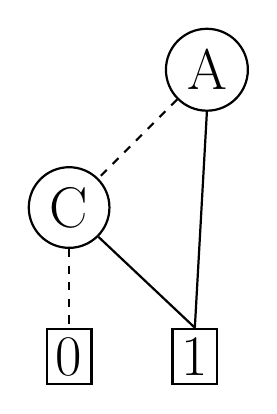
\begin{tikzpicture}
    \tikzstyle{inner} = [draw, solid, circle, thick];
    \tikzstyle{terminal} = [draw, solid, rectangle, thick];

    \node[inner] at (0, 0) (A) {\huge{A}};
    \node[inner, below left = 1 and 1 of A] (C) {\huge{C}}; 

    \node[terminal, below = 1 of C] (0) {\huge{0}};
    \node[terminal, right = 1 of 0] (1) {\huge{1}};

    \draw[thick, dashed] (A.south west) -- (C.north east);
    \draw[thick] (A.south) -- (1.north);

    \draw[thick, dashed] (C.south) -- (0.north);
    \draw[thick] (C.south east) -- (1.north);
\end{tikzpicture}

\end{document}